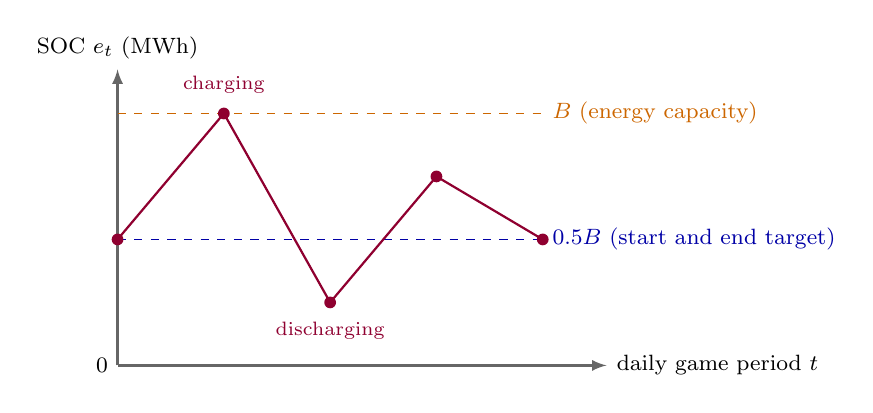
\begin{tikzpicture}[font=\footnotesize, >=latex, x=1.35cm, y=0.8cm]
  % Illustrative daily SOC path: starts and ends exactly at 0.5B.
  \tikzset{axis/.style={->, thick, draw=gray!80!black},
    point/.style={circle, fill=purple!75!black, inner sep=1.5pt}}
  \draw[axis] (0,0) -- (4.6,0) node[right] {daily game period $t$};
  \draw[axis] (0,0) -- (0,4.7) node[above] {SOC $e_t$ (MWh)};
  \draw[dashed, orange!80!black] (0,4) -- (4,4) node[right] {$B$ (energy capacity)};
  \draw[dashed, blue!65!black] (0,2) -- (4,2) node[right] {$0.5B$ (start and end target)};
  \node[left] at (0,0) {$0$};
  \draw[thick, purple!75!black] (0,2) -- (1,4) -- (2,1) -- (3,3) -- (4,2);
  \foreach \x/\y in {0/2,1/4,2/1,3/3,4/2} {\node[point] at (\x,\y) {};}
  \node[font=\scriptsize, text=purple!75!black, align=center] at (1,4.45) {charging};
  \node[font=\scriptsize, text=purple!75!black, align=center] at (2,0.55) {discharging};
\end{tikzpicture}
